\documentclass[border=2pt]{standalone}
\usepackage{amssymb,amsmath}
\usepackage{tikz-cd}
\usepackage{physics}
\usetikzlibrary{arrows}

\usepackage{tikz}
\let\OX\bigotimes
\newcommand{\OP}{\displaystyle\bigoplus}
\let\ox\otimes
\let\op\oplus
\let\isom\cong
\let\vf\varphi
\begin{document}

\tikzset{every picture/.style={line width=0.75pt}} %set default line width to 0.75pt        

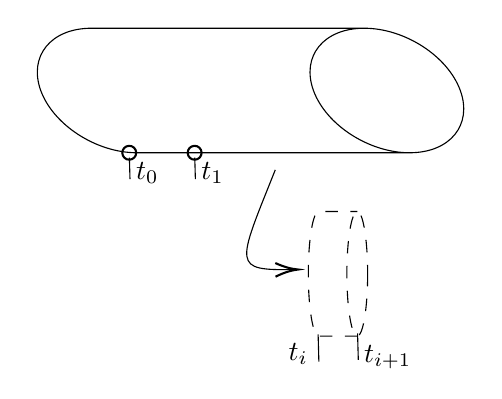
\begin{tikzpicture}[x=0.75pt,y=0.75pt,yscale=-1,xscale=1]
%uncomment if require: \path (0,241); %set diagram left start at 0, and has height of 241

%Flowchart: Direct Access Storage [id:dp5786229900826654] 
\draw   (210.68,98) -- (79.29,98) .. controls (59.76,98) and (39.03,84.57) .. (33,68) .. controls (26.97,51.43) and (37.92,38) .. (57.45,38) -- (188.84,38)(235.14,68) .. controls (241.17,84.57) and (230.22,98) .. (210.68,98) .. controls (191.15,98) and (170.42,84.57) .. (164.39,68) .. controls (158.36,51.43) and (169.31,38) .. (188.84,38) .. controls (208.38,38) and (229.11,51.43) .. (235.14,68) ;
%Straight Lines [id:da5893074994090735] 
\draw    (75.71,100.35) -- (76,110.75) ;
\draw [shift={(75.64,98)}, rotate = 88.4] [color={rgb, 255:red, 0; green, 0; blue, 0 }  ][line width=0.75]      (0, 0) circle [x radius= 3.35, y radius= 3.35]   ;
%Straight Lines [id:da19694637791321545] 
\draw    (107.21,100.35) -- (107.5,110.75) ;
\draw [shift={(107.14,98)}, rotate = 88.4] [color={rgb, 255:red, 0; green, 0; blue, 0 }  ][line width=0.75]      (0, 0) circle [x radius= 3.35, y radius= 3.35]   ;
%Flowchart: Direct Access Storage [id:dp15114335913071741] 
\draw  [dash pattern={on 4.5pt off 4.5pt}] (185.5,186.32) -- (166.91,186.32) .. controls (164.15,186.32) and (161.91,172.89) .. (161.91,156.32) .. controls (161.91,139.75) and (164.15,126.32) .. (166.91,126.32) -- (185.5,126.32)(190.5,156.32) .. controls (190.5,172.89) and (188.26,186.32) .. (185.5,186.32) .. controls (182.73,186.32) and (180.49,172.89) .. (180.49,156.32) .. controls (180.49,139.75) and (182.73,126.32) .. (185.5,126.32) .. controls (188.26,126.32) and (190.5,139.75) .. (190.5,156.32) ;
%Curve Lines [id:da5804114816457824] 
\draw    (146,106.25) .. controls (127.38,152.8) and (125.09,154.69) .. (155.12,154.28) ;
\draw [shift={(157,154.25)}, rotate = 539.1] [color={rgb, 255:red, 0; green, 0; blue, 0 }  ][line width=0.75]    (10.93,-3.29) .. controls (6.95,-1.4) and (3.31,-0.3) .. (0,0) .. controls (3.31,0.3) and (6.95,1.4) .. (10.93,3.29)   ;
%Straight Lines [id:da8081791899844226] 
\draw    (166.64,185.5) -- (167,198.68) ;
%Straight Lines [id:da7670770097216806] 
\draw    (185.64,185) -- (186,197.75) ;

% Text Node
\draw (77.64,101.4) node [anchor=north west][inner sep=0.75pt]    {$t_{0}$};
% Text Node
\draw (109.14,101.4) node [anchor=north west][inner sep=0.75pt]    {$t_{1}$};
% Text Node
\draw (151.14,188.78) node [anchor=north west][inner sep=0.75pt]    {$t_{i}$};
% Text Node
\draw (187.5,189.72) node [anchor=north west][inner sep=0.75pt]    {$t_{i+1}$};


\end{tikzpicture}
\end{document}